% 本文件保留历史实验的可核验摘要；详细实现、逐项推导和重复图形迁至代码仓库。
\section*{Original Experiments and Technical Details}
The following sections retain the protocols, principal results, and semantic
definitions needed to assess the original experiments. Extended derivations,
operator listings, complete plotting material, and implementation notes are
provided in \path{Docs/extended_materials/} in the anonymous repository.
The controlled measurements and application studies in
Appendices~\ref{app:revision_effects}--\ref{app:typed_graph_comparisons} retain their
separate protocols and execution-version records.

\section{Related Work and Representation Interfaces}
\label{sec:related_work}
Typed program graphs and reusable intermediate values are established in
strongly typed GP, CGP, and MT-CGP~\cite{montana1995strongly,miller2015cartesian,harding2012mtcgp}.
LLVM SelectionDAG separates typed data values from chain dependencies for
side-effect ordering~\cite{llvmSelectionDAG}. AdaptoFlux applies this separation
to a symbolic-synthesis interface: data edges bind arguments of registered
host-language callables, while the saved execution contract orders declared
conflicting resource accesses. Candidate evaluation, graph modification,
subgraph extraction, and persistence maintain that contract
(Appendix~\ref{app:revision_effects}).

DreamCoder learns reusable abstractions in a functional program
space~\cite{ellis2021dreamcoder}; mutable interaction can also be expressed by
passing explicit state values. Appendix~\ref{app:revision_encoding} compares
that interface with implicit accesses for the same programs and selected
access order. Popper learns logical programs through a
generate--test--constrain loop~\cite{cropper2021learning}; its failure-derived
constraints differ from the current supplied type declarations and search
metadata. These approaches provide alternative interfaces and search mechanisms,
rather than a separation in computability.

PySR, gplearn, and AI Feynman specialize in recovering numerical expressions
\cite{cranmer2023interpretable,udrescu2020ai}. Symbolic policy search and
language-model-guided discovery emphasize candidate generation and optimization
\cite{landajuela2021discovering,romera2024mathematical}. AdaptoFlux's common
registration and execution interface accommodates several such choices; the
current demonstrations use LayerGrow, GraphEvo, and a CMA-based controller
optimizer. Appendix~\ref{sec:appendix_baseline_comparison} retains the restricted
static-regression comparison, including its negative results.

\section{Execution and Search Cost}
\label{sec:complexity_analysis}
\subsection{Inference Cost}
\label{sec:single_inference}
For $V$ operation nodes, $E$ routed data edges, $N$ samples, and average operation
and routing costs $C_{\mathrm{op}}$ and $C_{\mathrm{route}}$, the original
backend separates input conversion, topological preparation, node execution,
and output aggregation. Topological sorting costs $O(V+E)$; executing a fixed
scalar graph contributes $O\bigl(N(VC_{\mathrm{op}}+EC_{\mathrm{route}})\bigr)$.
Input conversion and output aggregation additionally depend on input/output
size and the selected aggregation rule. These terms describe the original
backend used in the historical and Appendix~\ref{app:revision_scaling}
measurements.

The revised runtime prepares the saved semantic order and resource-control
dependencies before execution. Its scheduler operates on data and control
dependencies together. For stateful batches with effect ordering enabled, it
completes one sample's graph before the next; pure graphs use the batched
traversal. Section~\ref{subsec:inference_complexity} states this revised cost
decomposition. The original timings do not measure the new planning pass.

\subsection{Navigation Procedures}
\label{sec:detailed_analysis}
Search cost is the sum of candidate construction or modification, evaluation,
and acceptance/bookkeeping costs over the candidates actually examined.
LayerGrow repeatedly extends and evaluates a graph, with rollback after
unsuccessful proposals. Its growth-attempt cap therefore need not imply a
reached graph depth. GraphEvo evaluates replacements on a fixed skeleton and
can extract reusable subgraphs. CombinedTrainer alternates growth and
refinement with optional pool filtering. Candidate counts, graph sizes,
episode lengths, and stopping rules jointly determine their realized costs;
the protocols below retain these quantities separately from the type checks
and execution costs.

\subsection{Backend Constraints}
\label{sec:engineering_constraints}
Available concurrency is bounded by dependency width and critical-path length.
Thread-pool creation, ready-node management, Python dispatch, and intermediate
storage add backend costs. Simulated waiting operations and Python scalar
CPU operations exhibit different speedups (Appendices~\ref{sec:appendix_exp3}
and~\ref{app:revision_scaling}). Type compatibility checks do not detect
shared-state conflicts; those are governed by the separate execution contract.
Stage-by-stage cost derivations and profiling figures are retained in
\path{Docs/extended_materials/}.

\section{Original Experimental Protocols and Results}
\label{sec:appendix_experiments}
These experiments use the original backend. The following tables report their
original evaluation units and stopping criteria; they are not pooled with the
later controlled studies in Appendices~\ref{app:revision_types}--\ref{app:revision_capacity}.

\subsection{LayerGrow on Titanic}
\label{sec:appendix_exp1}
The historical runner loads preprocessed Titanic observations from
\path{train_processed.csv}; the reported accuracy is the search-time score on
the observations supplied to the trainer. This is a structural-exploration
probe rather than an independent generalization evaluation. The pool has
nine scalar operations: identity, two-output copying, addition, subtraction,
multiplication, protected division, increment, decrement, and negation.
Configured maximum depths are $5,10,\ldots,50$, with ten runs per setting,
ten attempts per layer, rollback by two layers, decision threshold zero, and
a total cap of 2,500 growth attempts. The historical seed expression is
$42r+\mathrm{hash}(\texttt{max\_layers\_}L)\bmod1000$ for $r=1,\ldots,10$;
reproduction therefore also depends on Python's hash initialization.

\begin{figure}[tb]
\centering
\begin{minipage}[t]{0.48\linewidth}
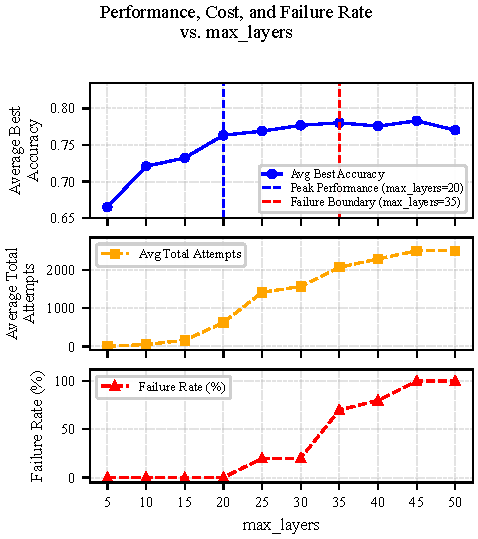
\includegraphics[width=\linewidth]{images/rebuttal_format/scaling_behavior_split.pdf}
\end{minipage}\hfill
\begin{minipage}[t]{0.48\linewidth}
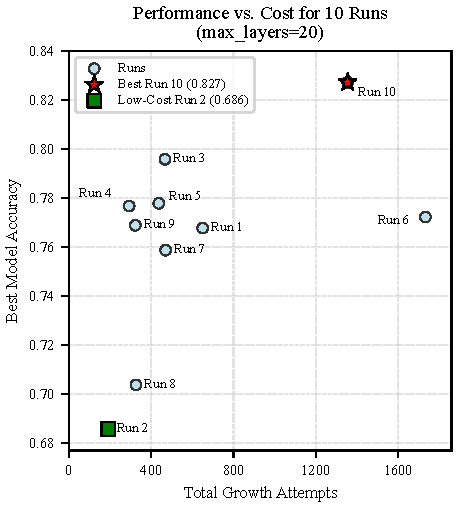
\includegraphics[width=\linewidth]{images/rebuttal_format/run_comparison_20.pdf}
\end{minipage}
\caption{Original LayerGrow study: configured-depth sensitivity and variation
among ten runs at a maximum of twenty layers. The configured maximum and
achieved depth are distinct.}
\label{fig:scaling_behavior}
\end{figure}

\begin{table}[tb]
\centering\small
\caption{LayerGrow results over ten runs per setting. Accuracy is the best
observed value per run, including runs stopped by the attempt cap. Exhaustion
means that all 2,500 attempts were consumed.}
\label{tab:convergence_stats_appendix}
\begin{tabular}{rrrrr}
\toprule
Max. depth & Accuracy (mean $\pm$ SD) & Reached depth & Attempts & Exhaustion (\%) \\
\midrule
5  & $0.665\pm0.042$ & 5.0  & 6.5    & 0 \\
10 & $0.721\pm0.030$ & 10.0 & 50.5   & 0 \\
15 & $0.732\pm0.036$ & 15.0 & 160.5  & 0 \\
20 & $0.763\pm0.041$ & 20.0 & 624.5  & 0 \\
25 & $0.769\pm0.028$ & 22.9 & 1414.9 & 20 \\
30 & $0.777\pm0.025$ & 26.3 & 1567.4 & 20 \\
35 & $0.780\pm0.022$ & 21.7 & 2069.2 & 70 \\
40 & $0.776\pm0.020$ & 23.3 & 2289.7 & 80 \\
45 & $0.783\pm0.024$ & 19.6 & 2500.0 & 100 \\
50 & $0.770\pm0.032$ & 18.7 & 2500.0 & 100 \\
\bottomrule
\end{tabular}
\end{table}

At requested depths 45 and 50, all runs exhaust the budget before attaining
those depths. This locates a search-budget bottleneck rather than failure to
execute a graph of that size. The source is
\path{experiments/LayerGrowTrainer_exp1/LayerGrowTrainer_exp1.py};
\path{main.py} in that directory aggregates the outputs. The configuration/run summary is
\path{experiment_results_summary.csv} in the same directory. Large per-attempt
logs are generated by the runner. Its historical runtime import requires the
matching original API when reproducing the experiment.

\subsection{GraphEvo and Reusable Subgraphs}
\label{sec:appendix_exp2}
The task chain is $f_1(x)=2(x+1)$, $f_2(x)=f_1(x)+3$, and
$f_3(x)=0.5f_2(x)$. All methods use scalar interfaces. The minimal pool contains
increment, multiply by two, add three, multiply by one half, and identity;
the extended pool adds \texttt{add\_2}, and the static-injection condition adds
the exact $f_1$ method to the minimal pool. There are 100 repetitions per
configuration, with NumPy seeds $42+\mathrm{rep\_id}$ and data resampled per repetition.
Tasks 1/2 use maximum initial depths two or three; Task~3 always permits at most three top-level calls.

Sample accuracy uses relative error below 1\%, with denominator
$|y|+10^{-8}$. Reported Task~3 success requires accuracy $>0.95$; the stricter
complete-chain criterion additionally requires Tasks 1/2 to reach accuracy
$\geq0.999$. The two counts are distinct.

\begin{table}[tb]
\centering\small
\caption{Original three-task reuse study, 100 runs per configuration. The
reported success criterion concerns Task~3. Static injection supplies $f_1$
directly; evolution extracts methods during training.}
\label{tab:exp3_results}
\begin{tabular}{llrrr}
\toprule
Pool updating & Pool & Task 1/2 depth & Task~3 accuracy & Successes/100 \\
\midrule
Disabled & Minimal & 2 & $0.0006\pm0.0021$ & 0 \\
Disabled & Extended & 2 & $0.0003\pm0.0012$ & 0 \\
Disabled & Minimal & 3 & $0.0007\pm0.0022$ & 0 \\
Evolution & Minimal & 2 & $0.1308\pm0.3360$ & 13 \\
Evolution & Extended & 2 & $0.1312\pm0.3359$ & 13 \\
Evolution & Minimal & 3 & $0.0908\pm0.2859$ & 9 \\
Static injection & Minimal+$f_1$ & 2 & $0.1206\pm0.3247$ & 12 \\
\bottomrule
\end{tabular}
\end{table}

\begin{figure}[tb]
\centering
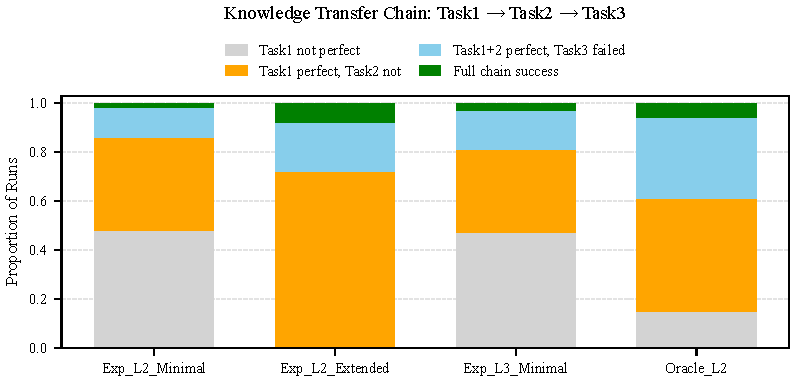
\includegraphics[width=0.70\linewidth]{images/rebuttal_format/exp3_knowledge_chain_from_logs.pdf}
\caption{Complete and partial transfer paths in the original three-task
experiment. Green denotes the stricter complete-chain criterion.}
\label{fig:exp3_chain}
\end{figure}

Exact enumeration shows that the fixed minimal and extended pools require four calls to express $x+2.5$. Composite methods can make it reachable within Task~3's three-call bound. The comparison therefore measures abstraction at fixed top-level depth; Appendix~\ref{app:typed_graph_comparisons} separately matches expanded capacity. Full-chain success remains limited. The implementation is
\path{experiments/GraphEvo_exp3/exp3_main.py}; configuration statistics are in
\path{exp3_results/summary_table.csv} below that directory. Complete model and
pool histories are regenerated by the script.

\subsection{Topology-Aware Task Parallelism}
\label{sec:appendix_exp3}
Thirty saved graphs from the LayerGrow study are evaluated using a dynamic
\texttt{ThreadPoolExecutor} with $1,2,4,8,16$ workers. Their actual depths span
2--35; graph identities and topology statistics are retained in the extended
material and the original benchmark records. The same input batch and method
pool are used across worker counts, with seed 42. Two workload modes are
distinguished: lightweight Python computation, and the same methods with a
1\,ms \texttt{time.sleep} inside each method to simulate non-blocking waiting.

For the waiting workload, shallow wide graphs attain a mean $10.25\times$
speedup with 16 workers. Across all 30 graphs at 16 workers, speedup correlates
with average width ($r\approx0.99$), whereas correlations with node count and
depth are approximately $-0.16$ and $-0.41$. These measurements characterize
the simulated waiting workload. The separate CPU experiment in
Appendix~\ref{app:revision_scaling} reports slower threaded execution for Python
scalar operations. Source configurations, the 30-graph inventory, structural
correlations, and profiling plots are available under
\path{experiments/PipelineParallel_exp2/} and \path{Docs/extended_materials/}.

\subsection{Original Minimal Stateful Synthesis Experiment}
\label{sec:appendix_exp4}
Position and target are drawn from $\{-2,-1,0,1,2\}$ with unequal initial
values. The graph rereads observations after each state-changing execution,
with at most four steps per episode. Each final graph is evaluated on 100
randomized episodes; a search run succeeds when at least 95\% reach the
target. Training probes use 20 episodes per evaluation. Both conditions use
seeds 42--51 and the same nine method implementations; only declared types and
the associated root-input signatures differ. The pool contains state readers,
direction calculation, the goal-aware movement operation, and distractors.

GraphEvo uses fixed three-layer initialization, three initial skeletons, up to
30 replacements per cycle and five cycles, the full candidate pool, disabled
method-pool evolution, and \texttt{early\_stop\_eps=0}. The reported graph is
the final graph of each search. These randomized ten-seed results are separate
from the exhaustive thirty-seed protocol in Appendix~\ref{app:revision_types}.

\begin{table}[tb]
\centering\small
\caption{Original stateful experiment: final success percentages over 100
episodes for each search seed. A successful search requires at least 95\%.}
\label{tab:stateful_per_run}
\begin{tabular}{lrrrrrrrrrr}
\toprule
Seed & 42 & 43 & 44 & 45 & 46 & 47 & 48 & 49 & 50 & 51 \\
\midrule
All scalar & 33 & 30 & 22 & 42 & 24 & 37 & 32 & 27 & 24 & 32 \\
Typed roles & 100 & 100 & 0 & 100 & 0 & 100 & 100 & 100 & 100 & 100 \\
\bottomrule
\end{tabular}
\end{table}

Typed roles succeed in 8/10 searches versus 0/10 for all-scalar declarations.
Mean final accuracies are $0.800\pm0.400$ and $0.303\pm0.060$, respectively.
The two typed failures omit the movement operation and never change state;
the scalar graphs contain movement but omit the intended direction calculation.
These observations isolate the supplied type-routing prior in this task.

\paragraph{Paired test and records.}
\label{sec:paired_test}
The shared seeds form ten pairs, with eight successes unique to the typed arm,
zero unique to the scalar arm, and two shared failures. The exact paired
McNemar test gives one-sided $p=2^{-8}=0.00390625$ and two-sided
$p=2^{-7}=0.0078125$. The configurations and per-run graphs are under
\path{experiments/minimal_stateful_comparison/};
\path{run_comparison.py} reproduces the comparison. The original source log is
\path{logs/experiment_log_20260920_124456.log} in that directory.

\section{Geometric Classification and Pool Composition}
\label{sec:appendix_geo_ablation}
The original study compares six search configurations on concentric circles,
two spirals with a full pool, and two spirals with a restricted pool. Each
configuration has 100 repetitions, seeds incremented from 42, 800 training
and 200 test examples, and standardized inputs. The restricted pool contains
15 scalar operations: the nine operations in Appendix~\ref{sec:appendix_exp1},
plus square, ReLU, absolute value, mean of three values, maximum, and minimum.
The full pool adds sine, cosine, \texttt{atan2}, protected square root, and scaling.

LayerGrow alone permits 15 layers; the other growth configurations permit
10, with a 250-attempt cap. GraphEvo alone permits ten rounds; the combined
conditions use eight refinement rounds per cycle. CombinedTrainer runs three
cycles. Pool filtering is disabled, applied once, or applied each cycle;
its target size is eight, population 20, elite fraction 30\%, mutation rate
15\%, and data fraction 30\%. Filtering uses four generations, reduced to two
in the periodic configuration. The stopping tolerance is $10^{-6}$.

\begin{table}[tb]
\centering\small
\caption{Original geometric-classification results: test accuracy (mean
$\pm$ SD) across 100 repetitions. ``Disabled'', ``once'', and ``periodic''
refer to pool filtering in the three-cycle CombinedTrainer.}
\label{tab:compact_geometry}
\begin{tabular}{lccc}
\toprule
Configuration & Circles & Spirals: full & Spirals: restricted \\
\midrule
Combined: disabled & $0.8909\pm0.0837$ & $0.8493\pm0.0338$ & $0.8386\pm0.0390$ \\
Growth then refinement & $0.7927\pm0.1354$ & $0.8148\pm0.0556$ & $0.7989\pm0.0421$ \\
Growth only & $0.7725\pm0.0622$ & $0.8053\pm0.0389$ & $0.8019\pm0.0355$ \\
Combined: once & $0.7472\pm0.1547$ & $0.7823\pm0.0793$ & $0.7791\pm0.0644$ \\
Refinement only & $0.6985\pm0.1080$ & $0.7624\pm0.0798$ & $0.7326\pm0.0992$ \\
Combined: periodic & $0.6292\pm0.1424$ & $0.7209\pm0.1094$ & $0.7381\pm0.0762$ \\
\bottomrule
\end{tabular}
\end{table}

The unfiltered combined configuration has the highest mean accuracy in all
three settings, but reaches 99\% test accuracy in only 24, 1, and 1 of the
100 runs. Thus the spiral tasks remain difficult despite the higher mean.
Training budgets and filtering schedules differ between configurations;
these results evaluate complete search configurations, not an isolated effect
of pool size. Detailed timings, selected graph plots, and decision-boundary
figures are retained in \path{Docs/extended_materials/}; scripts are under
\path{experiments/Combined_exp4_circles/},
\path{experiments/Combined_exp4_spiral/}, and
\path{experiments/Combined_exp4_spiral_no_Trigonometric/}.

\section{Static Symbolic Regression with Restricted Method Pools}
\label{sec:appendix_baseline_comparison}
Eight formula-recovery tasks compare the original probes with gplearn and
PySR~\cite{cranmer2023interpretable}, using arithmetic primitives
\texttt{add}, \texttt{sub}, \texttt{mul}, and \texttt{div}. ATF's construction
interface also supplies identity and copying operations. Output aggregation
is separately varied among \texttt{first}, \texttt{prod}, and \texttt{sum};
arbitrary imported methods and stateful actions are not used. Each condition
has ten independently seeded runs. The tasks are $mc^2$, $ma$, $0.5mv^2$,
$q_1q_2/r^2$, $nT/V$, $IR$, $(v_2-v_1)/t$, and $VI$.

\begin{table}[tb]
\centering\small
\caption{Best-of-ten test MSE in the original static-regression experiment.
Values retain the precision of the original summary tables.}
\label{tab:compact_regression_mse}
\begin{tabular}{lrrrrr}
\toprule
Task & ATF first & ATF prod & ATF sum & gplearn & PySR \\
\midrule
$mc^2$ & $2\mathrm{e}{+3}$ & $2\mathrm{e}{-11}$ & $8\mathrm{e}{+0}$ & $8.3\mathrm{e}{-12}$ & $8.3\mathrm{e}{-12}$ \\
$ma$ & $3\mathrm{e}{-12}$ & $2\mathrm{e}{-13}$ & $4\mathrm{e}{+1}$ & $1.9\mathrm{e}{-13}$ & $2.1\mathrm{e}{-12}$ \\
$0.5mv^2$ & $4\mathrm{e}{+3}$ & $2\mathrm{e}{-11}$ & $8\mathrm{e}{+2}$ & $3.4\mathrm{e}{-11}$ & $3.4\mathrm{e}{-11}$ \\
$q_1q_2/r^2$ & $1\mathrm{e}{+1}$ & $9\mathrm{e}{+0}$ & $1\mathrm{e}{+1}$ & $6.8\mathrm{e}{-14}$ & $2.7\mathrm{e}{-13}$ \\
$nT/V$ & $3\mathrm{e}{+4}$ & $2\mathrm{e}{+4}$ & $3\mathrm{e}{+4}$ & $1.0\mathrm{e}{-10}$ & $2.2\mathrm{e}{-10}$ \\
$IR$ & $5\mathrm{e}{-13}$ & $2\mathrm{e}{-13}$ & $1\mathrm{e}{-12}$ & $2.2\mathrm{e}{-13}$ & $2.2\mathrm{e}{-13}$ \\
$(v_2-v_1)/t$ & $7\mathrm{e}{+0}$ & $5\mathrm{e}{+0}$ & $1\mathrm{e}{+1}$ & $3.9\mathrm{e}{-14}$ & $1.1\mathrm{e}{-13}$ \\
$VI$ & $1\mathrm{e}{-12}$ & $8\mathrm{e}{-13}$ & $2\mathrm{e}{-12}$ & $8.0\mathrm{e}{-13}$ & $1.0\mathrm{e}{-12}$ \\
\bottomrule
\end{tabular}
\end{table}

\begin{table}[tb]
\centering\small
\caption{ATF numerical-match frequency across all ten runs. Numerical matching
requires absolute error below $10^{-5}$ on every test sample. This is distinct
from both MSE and the manual symbolic-equivalence check.}
\label{tab:compact_regression_success}
\begin{tabular}{lrrrrrrrr}
\toprule
Aggregation & $mc^2$ & $ma$ & $0.5mv^2$ & $q_1q_2/r^2$ & $nT/V$ & $IR$ & $(v_2-v_1)/t$ & $VI$ \\
\midrule
first (\%) & 0 & 20 & 0 & 0 & 0 & 10 & 0 & 50 \\
prod (\%) & 0 & 100 & 0 & 0 & 0 & 100 & 0 & 100 \\
sum (\%) & 0 & 0 & 0 & 0 & 0 & 20 & 0 & 30 \\
\bottomrule
\end{tabular}
\end{table}

The specialized symbolic solvers obtain much lower error on Coulomb, ideal-gas,
and acceleration tasks. ATF's product aggregation consistently recovers the
simple multiplication tasks, whereas the other modes have lower numerical-match
frequencies. Best-of-ten MSE alone therefore does not characterize robustness.
For the kinetic-energy task, the constant $0.5$ is supplied as an input feature.
Manual inspection classifies the best ATF product expressions as algebraically
equivalent for $mc^2$, $ma$, $0.5mv^2$, $IR$, and $VI$, but not for the other
three tasks. Numerical matching and symbolic equivalence use different criteria;
neither is substituted for the other.

The full expressions, run-level distributions, timing tables, XGBoost comparison,
and manual equivalence table are in \path{Docs/extended_materials/}. Executable
baseline scripts and result records are under
\path{experiments/ExternalBaselines/}. These restricted experiments evaluate
particular optimizers and aggregation rules; they do not establish a search
advantage of implicit state or of the representation over other typed graphs.

\section{Hand-Crafted Snake Controller}
\label{app:snake_controller}
The original untrained Snake controller reads observations, computes hazards
and food direction, and selects among \texttt{turn\_left}, \texttt{turn\_right},
and \texttt{go\_straight}. Mutually exclusive Boolean permits ensure that one
action updates the environment per tick. Numerical computation and action
emission share the stored graph; the graph is executed again on the next
observation. This illustrates the execution interface, independently of the
learned controllers in Appendix~\ref{app:revision_action}. The graph, demo,
and larger diagram are provided in \path{experiments/embodied_snake/} and the
extended material.

\section{Implementation and Reproduction Map}
\label{app:impl-details}
The \texttt{@method\_profile} decorator binds an implementation to positional
input/output signatures and metadata. Data ports determine argument routing;
\texttt{pure}, \texttt{reads}, and \texttt{writes} describe effects in the revised
runtime. The complete source interfaces are the executable reference, under
\path{ATF/methods/} and \path{ATF/GraphProcessor/};
\path{Docs/effect_execution_zh.txt} documents the optional effect-ordering mode.

\begin{table}[tb]
\centering\small
\caption{Repository entry points. Paths are relative to the anonymous repository;
each listed experiment retains its own configuration and output conventions.}
\label{tab:repo-mapping}
\begin{tabularx}{\linewidth}{@{}p{0.30\linewidth}X@{}}
\toprule
Study/material & Entry point or directory \\
\midrule
LayerGrow depth & \path{experiments/LayerGrowTrainer_exp1/} \\
GraphEvo reuse & \path{experiments/GraphEvo_exp3/} \\
Original parallelism & \path{experiments/PipelineParallel_exp2/} \\
Original stateful task & \path{experiments/minimal_stateful_comparison/} \\
Static regression & \path{experiments/ExternalBaselines/} \\
Four frozen V0 studies & \path{experiments/rebuttal_20261106/} \\
Extended technical material & \path{Docs/extended_materials/} \\
\bottomrule
\end{tabularx}
\end{table}

The four V0 studies supply a frozen runtime snapshot, source/protocol hashes,
raw records, an integrity verifier, and a launcher that writes reproduction
outputs into a new external workspace. The package README distinguishes
evidence auditing, execution replay, and fresh measurements. This preserves
the historical measurements when the repository runtime changes. The V1
regression suite and frozen-model replay are reported separately in
Appendix~\ref{app:revision_effects}. Large historical model dumps and per-attempt
logs are regenerated by their scripts; available summary records and selected
artifacts remain in the corresponding experiment directories.

\section{Method Metadata and Runtime Semantics}
\label{app:method-pool-semantics}
\subsection{Functional Tags}
Metadata may label a method as a numerical mapping, an action, or both. Such
descriptive tags support application-specific pool views. A method that returns
a value can still change state; a zero-output method can still perform an action.

\subsection{Reversibility Tags}
Tags describing invertibility or reversibility are optional search annotations.
They do not prove that a callable is invertible, determine its effect set, or
replace the runtime's execution contract. Extended illustrative taxonomies are
retained in the repository material.

\subsection{Task-Specific Pool Views}
A filter $\phi$ selects
$\mathrm{Q}_{\mathrm{view}}(\phi)=\{m\in\mathrm Q\mid\phi(\mathrm M_m)\}$.
The view changes the operators exposed to search, while sampling weights change
proposal probabilities within that view. Pool composition and search budgets
must therefore be recorded together when comparing outcomes.

\subsection{Hypothesis Class and the Formal Role of Metadata}
\label{app:metadata_role}
Equation~\ref{eq:expression_space} defines admissible data DAGs through port
compatibility and acyclicity. Filtering restricts that class to
$\Omega_{\mathrm{Q}_{\mathrm{view}},\Sigma}\subseteq\Omega_{\mathrm Q,\Sigma}$.
Stateful execution additionally depends on $P=(G,\pi,E_c)$: the frozen order
and control dependencies derived from declared resource accesses. Changing an
effect declaration can change the required schedule and hence the execution
contract; changing a search weight only changes proposal preference.

\begin{table}[tb]
\centering\small
\caption{Distinct roles of interface checks, effect declarations, and search metadata.}
\label{tab:hard-soft}
\begin{tabularx}{\linewidth}{@{}p{0.32\linewidth}X@{}}
\toprule
Mechanism & Role \\
\midrule
Port types and arity & Admit compatible data connections to argument positions. \\
Data-graph acyclicity & Admit a topological schedule for data dependencies. \\
Read/write resources and saved order & Preserve the chosen order of conflicting accesses when effect ordering is enabled. \\
Search tags and weights & Select and sample the methods considered by the optimizer. \\
Reuse metadata & Guide extraction and reuse; composite methods retain their effect contracts. \\
\bottomrule
\end{tabularx}
\end{table}

Type-prior measurements appear in Appendix~\ref{app:revision_types}; effect
validation appears in Appendix~\ref{app:revision_effects}. The pool-composition
studies evaluate complete search configurations rather than isolating only
the metadata filter.

\subsection{Root and Output Interfaces}
\label{sec:supp-boundary-nodes}
The root distributes the externally supplied input into declared typed ports.
The output interface applies a separately configured aggregation rule to its
incoming values, such as first output, sum, product, or identity. Aggregation
is configured through the collapse manager rather than selected from the
internal Method Pool. Its choice affects the represented input/output mapping
and is reported explicitly in Appendix~\ref{sec:appendix_baseline_comparison}.
State changes can occur at action nodes even when those nodes do not lie on a
path to an aggregated numerical output.

\subsection{Static Acyclicity and Runtime Loop Semantics}
\label{app:runtime_loops}
Let $P=(G,\pi,E_c)$ be a fixed successful per-step execution contract. Let the
state $s_t$ contain all persistent resources, and fix the input and random
choices for each step. One evaluation defines $\Phi_P$, and the next-observation
interface defines $\Pi$:
\begin{equation}
\label{eq:closed_loop}
s_{t+1}=\Phi_P(s_t,x_t),\qquad x_{t+1}=\Pi(s_{t+1}).
\end{equation}
The numerical graph output need not encode the entire environment state.

\paragraph{Finite-unrolling proposition.}
For finite horizon $T$, this trace has an equivalent acyclic unrolling using
$T$ copies of $G^+=(V,E_d\cup E_c)$, with complete state and observations carried
between successive copies.
\emph{Proof.} Within each copy, all dependencies point forward in $\pi$;
between copies, they point from step $t$ to $t+1$. Lexicographic order by
$(t,\text{position in }\pi)$ therefore orders every dependency forward.
Induction on $t$ establishes execution equivalence: identical initial state
and inputs yield the same first transition, and each subsequent copy receives
exactly the preceding state and observation. \hfill$\square$

The interaction loop is supplied outside the stored graph. A registered
callable may also invoke another graph or recurse internally; its outer effect
declaration must summarize the resources it accesses. Enclosing-graph type
checks do not prove termination or analyze arbitrary Python control flow.

\section{Challenges in Automated Synthesis of Stateful Policies}
\label{app:side_effect_experiments}
Early LayerGrow/GraphEvo control trials exhibited proxy-reward failures:
Snake policies repeatedly turned to survive without collecting food, while
Bird policies repeatedly jumped or failed to avoid obstacles. These exploratory
observations concern the tested pools, rewards, and search configurations;
they are separate from the formal minimal-stateful study and the later CMA
controller results. The public Snake directory contains the fixed demo, not
those training runs. The early Bird training code in
\path{experiments/embodied_bird/} is an implementation reference whose API may
require adaptation to newer runtime versions. Further qualitative notes are
retained in \path{Docs/extended_materials/}.

\section{Prospective Integration of Language-Model Candidate Generators}
\label{app:llm_candidate_generation}
A language model could propose graphs or graph edits from the task, registered
method interfaces, and graph schema. AdaptoFlux could validate method names,
arity, port types, and acyclicity, construct effect-control dependencies, and
execute the proposal to return task scores and trajectories. Executable-candidate
rate, task success, search budget, and generation/validation costs are suitable
evaluation measures. This propose--validate--execute--feedback integration is
a research direction, not a completed experiment.

\section{Limitations}
The original probes are sensitive to initialization, operator coverage,
aggregation, and credit assignment. Their results do not establish superiority
over other typed graph synthesis systems. Effect guarantees require complete
resource declarations and deterministic successful execution; static interface
checks do not verify arbitrary Python effects. The largest tested graph is not
a practical upper bound. The main-text limitations distinguish these issues
from the separate questions of explicit-state search and runtime preparation
cost.

\section{Broader Impacts}
\label{app:broader_impacts}
Inspectable program graphs can expose computations and action interfaces for
review, but interpretability does not itself ensure correct or safe behavior.
Registered methods may inherit data or design biases and may perform harmful
external actions. Applications should validate their Method Pool, isolate
execution where appropriate, and check action permissions and environment
constraints before deployment. The experiments use public numerical data and
synthetic environments, with no human-subject intervention.

\section{Discussion and Future Work}
\label{app:discussion_future_work}
\paragraph{Output interfaces.}
\label{subsec:rethinking_collapse}
The static-regression study shows that aggregation is part of the experimental
configuration. Future search procedures can optimize explicit output-producing
subgraphs while using identity aggregation, rather than assuming a fixed reducer.

\paragraph{Execution backends.}
\label{subsec:cpp_migration}
Compiled or hybrid backends may reduce interpreter, scheduling, and storage
costs. Their benefit must be measured against operator cost, graph concurrency,
and memory traffic; a change of implementation language alone does not establish
a speedup.

\paragraph{Reusable executable knowledge.}
\label{app:intended_use}
The controller and library studies provide concrete settings for combining
registered primitives with learned structure. Future work described in
Section~\ref{sec:conclusion} is to retain subgraphs with applicability conditions
and evidence, and revise them through interaction within bounded resources.
Broader transfer and continually learning behavior require their own
comparative evaluation.
